%!TEX root=../main.tex
\documentclass[../main.tex]{subfiles}
\begin{comment}
\addbibresource{../bib/bibliography.bib}
\end{comment}
\begin{document}
\subsection{Feature extraction of audio samples}
One very commonly used feature extraction method of audio files is Mel Frequency ceptstral coefficients (mffcc). The mffcs of a signal is a feature vector which describe the frequency components the signal is comprised of. Mffcs are used to describe audio signals and are commonly used when building deep networks for speech recognition. The main idea of mffcs is to squash the frequencies in a signal into Mel scale. The audio signal is firstly transformed into a discrete signal sampled at some frequency and the power spectrum (Discrete Fourier Transform) is computed for the signal. Mel filterbank is then applied to the power spectrum of the signal. Mel filterbank is a set of triangular shaped filters, usually 20-40 filters. The filter gives a response which resembles the Mel scale (1).
(1) F(Mel)=[2595*log10[1+f]700] 
The filtered signal is then transformed to the time domain using discrete cosine transform, and we get the mel frequency cepstral coefficients. The final output is k number of vectors where k is the number of mel filterbanks.\cite{martinez2012speaker}
\subsection{Speech recognition model}
The speech recognition is done with a k-layer neural network. The training of the network is done with mini-batch gradient descent and batch normalization is applied at each layer. During the training, cyclic learning rates \cite{cyclic} are used when updating the weights and biases of each layer. The cost is computed with cross-entropy loss. ReLu activation function was used at each layer. The weights are initialized with random numbers sampled from $\mathcal{N}(0,1/\sqrt{m^{l-1}})$ where $m^{l-1}$ is the number of nodes in the previous layer. The biases are initialized to vectors containing zeros. When training with cyclic learning rates, the learning rate varies linearly between a specified lower and upper boundary for a specified number of cycles. The table below describes the hyperparameters of minibatch gradient descent along with cyclic learning rates.

\begin{center}
\begin{tabular}{|c c|} 
\hline
\textbf{Parameter} & \textbf{Description}\\ [0.5ex] 
 \hline\hline
$\eta_{min}$ & the lower boundary for cyclic learning rate \\  \hline
$\eta_{max}$ & the upper boundary for cyclic learning rate \\
\hline
n_s & is the stepsize of the cyclic learning rate.\\ & $2n_s$ corresponds to a whole cycle with\\ & $2n_s$ update steps \\
\hline
 \lambda & is the degree of regularization that is used \\
 \hline
 $n_{batch}$ & is the size of the batch in minibatch \\ &  gradient descent \\  
 \hline
$l$ & is the number of cycles for learning rate, \\ & i.e. the network is trained for in \\ & total $l*2*n_s$ update steps \\ [1ex]
\hline
\end{tabular}
\caption{Table 1}
\end{center}

\subsection{Text Encoding}
The text embedding, $\varphi(t)$, of the text description is generated by a pre-trained encoder \cite{reed2016learning}. We used a word2vec \cite{mikolov2013word2vec} model trained on 3.3 billion Google news articles. Every caption is fed word for word into this model to yield a 300-dimensional feature space text embedding. Because of the captions' different length we calculate the $max$ and $min$ elements row-wise in the sentence. These vectors are then stacked into a text embedding of length 600. This yields an adequate feature space representations for short sentences \cite{de2016representation} although the sentence structure is lost.
In other work the output has been averaged \cite{reed2016learning} or only used a simple bag of words model, thus order is deemed non-essential for the success of the network.
\subsection{Image Generation}
The image generation is done with a Conditional GAN \cite{mirza2014conditionalgan} with small perturbation to the condition variable. In \cite{zhang2017stackgan}, condition augmentation is used in which instead of just using the fixed text embedding $c = \varphi(t)$, they sample the latent variables $\hat{c}$ from a normal distribution $\mathcal{N}(\mu (c),\Sigma (c))$, where $\Sigma (c)$ is the diagonal covariance matrix. This sampling mitigates discontinuity in the latent data manifold and therefore makes training process more manageable. We approximate this behaviour by adding a small perturbation $p$, to the condition variable which is sampled from a normal distibution $\mathcal{N}(0,0.001)$ for which $\hat{c} = c + p$. Since a property of the text embedding is that words with similar meaning are similar in feature space this should also help generalize the output of the network.

The latent vector $z$ is sampled from $\mathcal{N}(0,1)$ and has a length of 64. 
\begin{figure}[h]
    \centering
    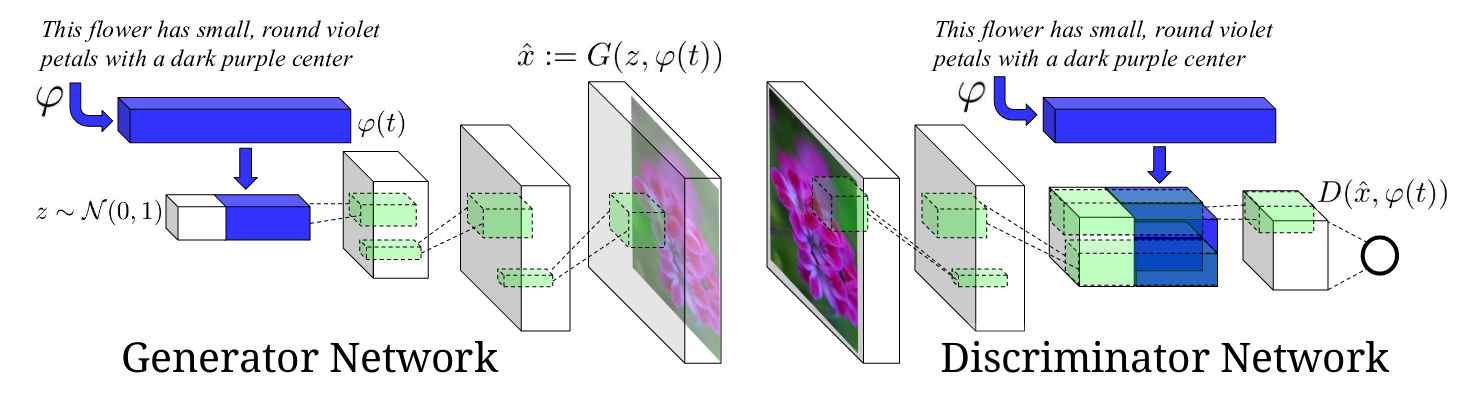
\includegraphics[width=\textwidth]{network_structure.png}
    \caption{Overall network structure of the image generation. Image from \cite{reed2016generative}}
    \label{fig:overall_structure}
\end{figure}
\subsubsection{Generator}
As seen in the left part of Figure \ref{fig:overall_structure}, the latent vector $z$ is appended to $\hat{c}$ and fed into the network. The input vector is upscaled to $\mathbb{R}^{512 \times 4 \times 4}$ with transposed convolution and batch normalization with a Relu activation function. This is repreated for dimensions $\mathbb{R}^{256 \times 8 \times 8}$, $\mathbb{R}^{128 \times 16 \times 16}$, $\mathbb{R}^{64 \times 32 \times 32}$ and $\mathbb{R}^{3 \times 64 \times 64}$ with tanh as activation function for the latter. The output is our $64 \time 64$ image with three color channels. Every convolution layer has a kernel size of 4 and stride of either 1 or two, depending on the layer in question.
\subsubsection{Discriminator}
The Discriminator can be seen to the right of Figure. \ref{fig:overall_structure}. It consists of 4 convolution layers for the input image. There is also a leaky-ReLu after every layer with an incline of 0.2. These convolution transform the $64 \times 64$ image into $\mathbb{R}^{64 \times 32 \times 32}$, $\mathbb{R}^{128 \times 16 \times 16}$, $\mathbb{R}^{256 \times 4 \times 4}$. Kernel size is 4 and stride is 2. 
At this point the discriminator does an 1d convolution of the text embedding and reshapes it to append to the current state of the image convolution. This stack is then fed into a convolution layer with 1 as output dimension. The activation function for this layer is a sigmoid function. 

\subsubsection{Training process}
The discriminator needs to be able to distinguish generated images from real ones, but it also need to be able to determine if the text embedding is representative of the depicted scene. The discriminator will thus be given three different kinds of input during training: Real image with real text ($s_r$), Real image with wrong text ($s_w$) and fake image with real text($s_f$). The generator thus has the following loss function. 
\begin{equation}
    \mathcal{L_D} = log(s_r) + \frac{1}{2} \left( log(1 - s_w) + log(1-s_f)\right) 
\end{equation}
The generator simply has to create the best fake images possible and has the loss function 
\begin{equation}
    \mathcal{L_G} = log(s_f)
\end{equation}
The training was done in minibatches with 64 images in each using the ADAM optimizer with a step size of 0.0002. A simplified view of the training algorithm can be seen in Table \ref{alg:gan}.
\begin{algorithm}[h]
\SetKwInOut{Input}{Input}
\SetKwInOut{Output}{output}
\SetAlgoLined
\Input{ Minibatch images $x$, Minibatch text embeddings $\varphi(t)$, number of training batch steps $S$}\\
\For {$i = 1$ to $S$}{
    $z \sim$  $\mathcal{N}(0,1)^Z$ \{Generate latent vector\}\\
    $p \sim$ $\mathcal{N}(0,0.001)^{\phi}$ \{Generate perturbation vector\}\\
    $w \sim$ $\mathcal{N}(0,1)^{\phi}$ \{Generate wrong text embedding\}\\
    $\hat{c} \leftarrow \varphi (t) + p$ \{Perturb text embedding\}\\
    $\hat{x} \leftarrow G(z, \hat{c})$ \{Generate fake image\}\\
    $s_r \leftarrow D(x,\hat{c})$ \{Real image, Real text\}\\
    $s_w \leftarrow D(x,w)$ \{Real image, Wrong text\}\\
    $s_f \leftarrow D(\hat{x},\hat{c})$ \{Fake image, Real text\}\\
    $\mathcal{L_D} \leftarrow log(s_r) + (log(1 - s_w) + log(1-s_f))/2$ \\
    $D \leftarrow D - \alpha \partial \mathcal{L_D} / \partial D$ \{Update discriminator\}\\
    $\mathcal{L_G} \leftarrow log(s_f)$\\
    $G \leftarrow G - \alpha \partial \mathcal{L_G} / \partial G$ \{Update generator\}\\
}
\caption{The training algorithm for the image generation, using Mini batch SGD with step size $\alpha$ for simplicity.}\label{alg:gan}
\end{algorithm}
The image generation was written from scratch in PyTorch and trained on a NVIDIA Tesla K80 GPU for approximately 28 hours, or 100 epochs, on the \texttt{flickr\_30k} dataset. The GAN has thus been trained on around 15 million different text and image combinations. 
\end{document}
